%\stepcounter{contsubsec} 
\section{INTRODUCCIÓN}

La determinación y el control de actitud en satélites son esenciales para el éxito de una misión espacial. Existen diferentes métodos de control de actitud, los cuales pueden clasificarse como pasivos y activos. El control pasivo recurre principalmente al diseño geométrico y magnético del satélite, buscando aprovechar los principios físicos y fuerzas naturales que actúan sobre el satélite, aumentando los efectos de una mientras se minimizan los de otras. Por otro lado, el control activo emplea actuadores como propulsores, magnetorquers (barra de torsión) o ruedas de reacción (Reaction Wheels, RW)  para modificar la actitud del satélite mediante la generación de torques correctivos \cite{Wertz1999}. Durante una misión espacial, se pueden utilizar diferentes modos de control de actitud para sus diferentes fases y tareas del satélite.
En los últimos años, se ha presentado un aumento de misiones espaciales que involucran CubeSats, el cual es un tipo de nanosatélite formado a partir de unidades cúbicas (U) de 10 cm de lado, y que cada vez presentan una mayor complejidad. Por lo tanto, ha sido de gran interés el incremento de la vida útil y el rendimiento de las misiones, donde el sistema de determinación y control de actitud (Attitude Determination and Control System, ADCS)  juegan un papel fundamental para garantizar la probabilidad de éxito \cite{Venturini2018}. En este sentido, el control de actitud de un CubeSat es fundamental para cumplir el perfil de misión, normalmente situado en órbita baja (Low Earth Orbit, LEO),  donde se busca tener precisión de apuntamiento y estabilidad para las cargas útiles, antenas y paneles solares, que son componentes críticos para el funcionamiento de la nave espacial y del éxito de la misión.
El control de actitud en CubeSats es normalmente provisto por RW, las cuales intercambian momento con la nave sin consumir propelente. No obstante, una desventaja de este tipo de dispositivos electromecánicos es que acumulan el momento para mantener una actitud deseada y, en consecuencia, las RW se saturan cuando alcanzan su velocidad máxima de rotación lo cual impiden que estas puedan intercambiar momentos que garanticen a la estabilidad del satélite. Por tal motivo, surge un desafío en el área de control de actitud que busca la desaturación de dichas ruedas de reacción mientras se conserva la actitud del satélite.
Algunos de los desafíos que se presentan frente a este fenómeno se deben a que comúnmente el control de actitud y la desaturación de RW son tratados por separado, y a pesar de que existen numerosos estudios sobre el control de actitud con torques magnéticos, hay pocos artículos que involucran la desaturación del momento de las RW mediante magnetorquers \cite{Yang2017}. Por otro lado, se requieren controladores que garanticen la estabilidad del satélite anticipando y actuando ante perturbaciones presentes en el ambiente espacial como por ejemplo torques externos debido a gradientes gravitacionales, torques aerodinámicos o torques de radiación solar \cite{Kaplan1976}.
Debido a esto, es de particular interés estudiar técnicas de desaturación con controladores, que permitan asistir estos dispositivos recurriendo a otros actuadores auxiliares como los magnetorques, los cuales, por medio de su interacción con campos magnéticos, generan un par que desatura las ruedas de reacción. No obstante, a diferencia de las RW que pueden generar un torque en cualquier dirección y en cualquier momento, los magnetorques dependen de la interacción con el plano ortogonal del campo geomagnético instantáneo, el cual cambia a medida que el satélite orbita alrededor de la tierra \cite{Tregouet2015}. Adicionalmente, a pesar de que los magnetorques son dispositivos confiables en LEO, producen una respuesta más lenta en comparación con otros actuadores lo cual reduce la capacidad de maniobra del satélite y su tiempo de reacción ante perturbaciones externas.
En este sentido, se propone evaluar estrategias de control de actitud que incorporen la desaturación de las ruedas reacción, mediante simulaciones computacionales a partir de un modelo dinámico basado en el CubeSat de entrenamiento EyasSat \cite{Eyassat}. Adicionalmente, se pretende realizar una comparación de diferentes controladores bajo algunos escenarios o perfiles de misión propuestos, con el fin de determinar las condiciones donde mejor se desempeñan las estrategias de control propuestas. La elección de este modelo en particular de CubeSat se debe a que dicho satélite se encuentra disponible en el programa de Ingeniería Aeroespacial; y es de especial interés incluirlo en el planteamiento de las simulaciones porque puede ser aprovechado junto con otros equipos, como la Jaula de Helmholtz, para consolidar una futura línea de investigación en control satelital.


\newpage
%--------------------------------------------

%Las \section{} que para esta plantilla son los títulos de nivel 1 siempre inician en una página nueva. Las \subsection{} y demas particiones de niveles 2 al 4 pueden ir en medio de una página.

\section{PLANTEAMIENTO DEL PROBLEMA}

%Se refiere al interrogante que lleva al investigador a buscar respuestas concretas. Es la definición del problema que aborda con la investigación. 

Estrategia de control que  permita eliminar la saturacion de la rueda de reacción 

\begin{figure}[!ht]
	\begin{center}
		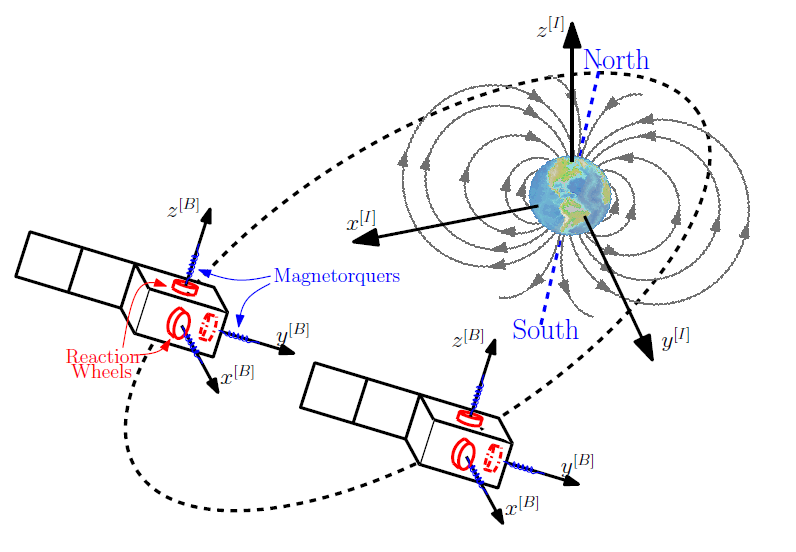
\includegraphics[scale=0.5]{imagenes/modelo_dinamico/diagrama_problema.PNG}\\
	\end{center}
	\caption{An inertially pointing satellite orbiting around the earth and equipped
		with reaction wheels and magnetorquers.}
	\label{diagrama_problema}
	\footnotesize{Nota. Fuente \url{https://www.ieee.org/}.} %\citep{lib:apa}.
\end{figure}

\subsection{Estado del Arte}

La desaturación de ruedas de reacción es un problema común en los satélites, incluidos los Cubesats, que pueden llevar a una pérdida de control de actitud. La ley de producto cruzado (CCPL) es una solución clásica en ingeniería comúnmente utilizado para resolver este paradigma desde una aproximación lineal \cite{Tregouet2015}. Pero en los últimos años se han desarrollado diferentes controladores que involucran sistemas no lineales.
Sin embargo, tal como se expresa en \cite{Yang2017}, el problema de control de actitud y la saturación de ruedas de reacción es comúnmente abordado como temas separados desde el punto de vista de diseño, por lo cual, no existen tantos artículos en los que se incluyan ambos objetivos. En su trabajo se propone un método de diseño de un LQR periódico variable en el tiempo donde se incluyen los torques generados por gradientes gravitacionales y los efectos periódicos del campo geomagnético alrededor de la órbita. Además, señala que los artículos existentes no suelen estos efectos mencionados anteriormente.
Por otro lado, Yang menciona esfuerzos como el de \cite{Tregouet2015} , en el cual se estudió al mismo tiempo el problema de la estabilización y el de desaturación de ruedas de reacción. A su vez se consideró la variación temporal del campo magnético en el marco del cuerpo (BRF), y su marco de referencia era el marco inercial (ECI). Sin embargo, para una nave espacial en LEO que utiliza el campo geomagnético, el marco de referencia más idóneo es el marco local vertical local horizontal (LVLH). Además, su diseño se compone de dos bucles, que es esencialmente una idea de tratar con el control de actitud y la desaturación en consideraciones separadas.
En esa misma línea, de Angelis \cite{Angelis2016} propuso un controlador proporcional heurístico y utilizó una función de Lyapunov para probar que el controlador puede simultáneamente estabilizar la nave espacial con respecto al marco LVLH y lograr la desaturación de ruedas de reacción. Pero este método de diseño no tiene en cuenta el efecto variable en el tiempo del campo geomagnético en el marco del cuerpo.
Finalmente, al estudiar las estrategias de control ya implementadas y conocer, tanto los efectos que incluyen como las simplificaciones de sus sistemas, es necesario recurrir a un modelo dinámico del EyasSat, el cual es el punto de partida para diseñar los controladores que se evaluarán bajo las condiciones de saturación y de estabilidad. A pesar de, no encontrar modelos dinámicos específicos para el EyasSat, Groenewald y Steyn \cite{Groenewald2014} elaboraron una propuesta para un nuevo ADCS integrado en este cubesat, y en él se incluyen propiedades inerciales y dimensiones útiles para la formulación de un modelo dinámico.
A su vez, en \cite{tes:Sorolla2019} se realiza un desarrollo matemático de la dinámica de un cubesat de 1U, donde describe los diferentes torques y perturbaciones externas, modela los actuadores en Simulink y sus diferentes configuraciones para ser evaluados bajo diferentes condiciones como la desaturación de ruedas de reacción.


\newpage
%-------------------------------


\section{JUSTIFICACIÓN}

Responde a los interrogantes del por qué se desea conocer el tema y por qué se seleccionó, así como cuál es el aporte que tendrá el texto a la ciencia. 

No abuse del uso de \textit{cursivas} o \textbf{negritas} dentro del texto, úselas muy moderadamente, por lo general saturan y dificultan la lectura del documento. Utilice cursivas en casos muy particulares como géneros y especies (\textit{Tyrannus melancholicus}), términos químicos (\textit{kr}), letras griegas ($\beta$) y algunos títulos y subtítulos. El entorno matemático de \LaTeX \ muestra las variables y símbolos en letra cursiva, asegurese de hacer lo mismo al referenciarla en el documento, Utilice \textbf{negritas} en algunos títulos de capítulos y subcapítulos, algunos datos de tablas o enfatizar aspectos muy particulares. El uso de \underline{texto subrayado} no se recomienda en normas IEEE.

Utilice moderadamente el uso de abreviaturas, se prefiere que el texto sea más largo y claro que corto y confuso para el lector. Por ejemplo, IEEE puede significar Institute of Electrical and Electronics Engineers o Instituto Español de Estudios Estratégicos. Sin embargo, las abreviaturas pueden ser útiles en casos como la repetición continua en un mismo párrafo.

Prefiera las comillas “inglesas” y ‘sencillas’ por sobre las «latinas» o «españolas».

\begin{description}
    \item[Características:] texto descriptivo.
    \item[Propiedades:] texto descriptivo.
    \item[Estructura:] texto descriptivo.
\end{description}

\newpage
%--------------------------
\section{OBJETIVOS}

\subsection{Objetivo general}



%El objetivo general y los objetivos específicos describen lo que se pretende con la investigación, cuál es el alcance y cuál es el problema que se desea resolver. Deben iniciarse con verbos que describan claramente lo que se lleva a cabo.
Validar computacionalmente una estrategia de control de actitud para el picosatélite CubeSat EyasSat que integre la desaturación de sus ruedas de reacción mediante magnetorquers a partir de su modelo dinámico.

\subsection{Objetivos específicos}

%Se describen algunos ejemplos de verbos comunes que se utilizan en el planteamiento de objetivos, los cuales cambiarán dependiendo de su investigación.
\begin{itemize}
\item Simular el comportamiento dinámico del nanosatélite EyasSat a partir del desarrollo de un modelo fenomenológico de este.
\item Determinar una estrategia de control de actitud para el nanosatélite EyasSat que integre la desaturación de las ruedas de reacción empleando magnetorquers a partir de simulaciones computacionales basadas en su modelo dinámico. 
\item Identificar aquellas órbitas donde la estrategia de control presente el mejor desempeño al utilizar los magnetorquers como elementos de desaturación de las ruedas de reacción.

\end{itemize}


\newpage
%--------------------------
\section{PROBLEMA DE INVESTIGACIÓN}

El problema de investigación es el enunciado de lo que puede ser demostrado o encontrado, y de lo cual se requieren pruebas y evidencias.



        

\newpage
%--------------------------
\section{MARCO TEÓRICO}

En esta sección se citan los autores que han tenido influencia directa en tu investigación. Recuerda, debes escoger solo un método para realizar las citas y referencias, es decir, debes seleccionar entre gestores especializados como Mendeley, Zotero, EndNote, etc., Microsoft Word, o “Manuales”; no se deben mezclar entre sí. Nuestra recomendación principal es Mendeley. Evita referenciar sitios como blogs, Wikipedia, Rincón del Vago, Monografías.com y demás portales web que no se consideran fuentes primarias. No limites tu búsqueda a una sola herramienta (por ejemplo, solo www.google.com). Realiza búsquedas en diferentes plataformas académicas, tales como:

\begin{itemize}
    \item \textbf{Catálogo Sistema de Bibliotecas UdeA:} material impreso que reposa en Bibliotecas UdeA, tales como libros, revistas, tesis, diccionarios, informes, etc.
    \item\textbf{Bases de datos suscritas de la Biblioteca:} plataformas digitales con millones de documentos en texto completo.
    \item\textbf{Bases de datos de libre acceso:} Google Scholar, Microsoft Academic, Google Books, Redalyc, Scielo, Dialnet, DOAJ, PubMed, Base Search, entre muchas más.
    \item\textbf{Documentos con acceso restringido:} si requieres el texto completo de artículos o libros con acceso restringido, que por lo general se encuentran en bases de datos no suscritas por la Universidad de Antioquia, solicítalos en tu Biblioteca enviando título exacto, el DOI o la url del documento. Tenemos convenios nacionales e internacionales que nos permiten acceder a esta información.
\end{itemize}

Ejemplo de cita parafraseada, es decir, frase no textual adaptada con las palabras de quien escribe; esta forma de citación es la más adecuada en textos académicos, demuestran lectura, análisis y redacción propia \cite{sec:pediatria}. Ejemplo de “Cita textual menor a 40 palabras, al interior del párrafo; no utilice recurrentemente esta forma de citación, pues demuestra poco análisis y redacción propios” \cite[p. 9]{opc:ramirez}. Otros ejemplos aceptados en estilo IEEE 2020:

En citas paráfrasis, es posible mencionar o no el o los autores en la oración, ejemplos: resultados demostrados por Arango \cite{sec:pediatria}, resultados demostrados mediante publicación científica \cite{sec:pediatria}. Cita en paráfrasis de dos autores, con o sin autor mencionado: datos suministrados por Ramírez y Guzmán \cite{opc:ramirez}, datos suministrados en revista académica \cite{opc:ramirez}. Cita en paráfrasis con tres o más autores con et al.: resultados publicados por Baker et al. \cite{art:baker}, resultados publicados en revista científica \cite{art:baker}. Cita con dos fuentes, cada una en corchetes y en orden numérico: ambos autores coinciden en estos datos \cite{opc:bbva}, \cite{opc:film}. Cita con tres fuentes o más, con corchetes para el primero y el último, en orden numérico y separados por guion: diversos autores coinciden en estos datos \cite{opc:bbva}–\cite{lib:ieee}. 

Cita “textual menor a 40 palabras” \cite[p. 466]{art:espectador}, cita “textual menor a 40 palabras con páginas continuas o discontinuas” \cite[pp. 15-16]{tes:tesis}.  %[8, pp. 15-16). debe terminar en parentesis

Cita de cita en paráfrasis mencionando o no autores: Quintero y González, citados por Rioja \cite{con:conferencia}, Quintero y González, citados por \cite{con:conferencia}. Cita textual mayor a 40 palabras sin comillas:


    \begin{quotation}
    Es importante destacar que la revisión realizada permitió definir el constructo a evaluar, es decir, especificar el concepto de la e-inclusión que se asume en la investigación, así como los factores que deben ser considerados para su evaluación. Lo anterior constituye el fundamento conceptual de la tesis y es la base para desarrollarla \cite[p. 107]{art:acimed}. 
    \end{quotation}

Cita textual o directa con más de 40 palabras (se omiten las comillas), bloque aparte, sangría 1.25 cms. Ya que IEEE no señala nada en particular de este caso, se adaptan de las normas APA. Datos estadísticos analizados con SPSS \cite{opc:ibm}. Procure no incurrir en la citación excesiva: 

\newpage
%--------------------------
\subsection*{MÉTODO PARA ELABORAR CITAS Y REFERENCIAS}

Recuerda, debes escoger solo un método para realizar las citas y las referencias, es decir, debes seleccionar entre un gestor especializado como Mendeley, Zotero o EndNote (confiabilidad alta), el gestor nativo Microsoft Word (confiabilidad media) o “manuales” (confiabilidad baja); no se deben mezclar entre sí, nuestra recomendación principal es Mendeley, pues te permite almacenar, subrayar e insertar notas en PDF´s, guardar fichas bibliográficas, elaborar citas y bibliografías en APA, Vancouver, IEEE y más de 1.000 estilos diferentes, exportar registros, compartir documentos, etc. Para mayor información de Mendeley.com y \LaTeX visitar:

\url{http://tiny.cc/zzrnuz}

La presente plantilla incluye los archivos requeridos para la construcción apropiada de las referencias bibliograficas bajo los parametros de las normas IEEE, todo se limita a modificar los campos del archivo \textit{refe.bib} segun las necesidades de su escrito. Aqui algunos ejemplos de los diferentes tipos de documentos referanciables.


Refencia a un libro \cite{lib:libro}, a un artículo \cite{art:baker}, a una seccion de libro sin título \cite{sec:pediatria}, a un acta \cite{act:acta}, a una conferencia \citep{con:conferencia}, a un capítulo o páginas específicas con título propio de un libro\citep[pp. 7-10]{ent:entre_libro},  a un documento sin editorial \citep{fll:folleto}, a las memorias de una conferencia \citep{ina:articulo_en_acta}, a un informe técnico \citep{inf:informe_tecnico}, a un manual \citep{man:manual}, a una tesis doctoral \citep{phd:phd_tesis}, a una tesis de maestría \citep{tes:tesis}, a una web o información de internet \citep{web:web} y para otros tipos de referencias diferentes a las anteriores \cite{opc:film}. Para el listado de referencias, tenga en cuenta que el apellido principal será la última palabra en el campo \textit{author}; Si como autor no figura una persona sino una organización, al llenar el campo \textit{author} del archivo \textit{.bib}, use $\{\}$ dobles (ver referencia \citep{lib:ieee}).

A continuación se muestra una de las referencias del archivo \textit{refe.bib}, donde \linebreak \textit{ent:entre\_libro} es el identificador de la misma y para referenciarla se debe escrbir el comando $\backslash cite\{ent:entre\_libro\}$ 

\newpage
\begin{verbatim}
@inbook{ent:entre_libro,
     author         = {Angela Zapata},
     title          = {Titulo de libro},
     chapter        = {},
     pages          = {10-20},
     publisher      = {Editor},
     volume         = {},
     series	        = {},
     type           = {},
     address        = {},
     edition        = {},
     year           = {20XX},
     month          = {},
     note           = {},
     language       = {},
     }
\end{verbatim}

Recuerde que \LaTeX , en la sección de referencias, solo muestra las que se han citado en su escrito; agregar la información en el archivo \textit{refe.bib} no implica que la referencia se muestre en su documento

Por otro lado, para citar ecuaciones e información semejante dentro del texto use $\backslash ref\{\}$, por ejemplo (\ref{eq:maxwell}) o (\ref{eq:maxwell3})

\begin{equation}\label{eq:maxwell}
    \oint_C \vec{B}\cdot d \vec{l}=\mu_0\int_S \vec{J}\cdot d \vec{s}+\mu_0\epsilon_0\dfrac{d }{d t}\int_S \vec{E}\cdot d \vec{s}
\end{equation}

y a su vez

\begin{gather}
    \vec{\nabla}\cdot \vec{E}= \dfrac{\rho}{\epsilon_0}\\
    \vec{\nabla}\cdot \vec{B}= 0\\
    \vec{\nabla}\times\vec{E}=-\dfrac{\partial\vec{B}}{\partial t}\\
    c^2\vec{\nabla}\times\vec{B} =\dfrac{\vec{J}}{\epsilon_0}+\dfrac{\partial
\vec{E}}{\partial t}\label{eq:maxwell3}\\
    \vec{\nabla}\times \vec{B}=\mu_0\vec{J}+\mu_0 \epsilon_0 \dfrac{\partial \vec{E}}{\partial t}
\end{gather}


\newpage
%--------------------------
\section{METODOLOGÍA}

%En la metodología se establecen los enfoques de investigación, esto es, cuantitativo, cualitativo o mixto.
La estrategia metodológica tiene un enforque cuantitativo, ya que toma como punto de partida un fenómeno, que puede ser amplio en el campo de la dinámica de satélites, pero que se acota cada vez más según se definen las preguntas de investigación, su alcance y su definición de variables. Por otro lado, se define un conocimiento mínimo, consolidado en el marco teórico, y una revisión de los métodos e investigaciones que se han realizado hasta el momento, consignado en el estado del arte.
En este sentido, el desarrollo de este trabajo de grado se divide en tres etapas:
\subsection{Modelo dinámico} 
Primero es necesario interpretar el fenómeno de estudio, partiendo de la realidad y llevándola a un entorno matemático que permita su simulación. Para ello se recurre a un modelo dinámico, constituido por las ecuaciones diferenciales involucradas en el fenómeno físico y sus propiedades inerciales.
De esta manera se pretende resolver las siguientes preguntas: ¿Cuál es el marco de referencia idóneo para plantear las ecuaciones del modelo dinámico? ¿De qué manera se puede comprobar que el modelo dinámico se acerca al modelamiento real del fenómeno? ¿Qué torques internos y externos deben tenerse en cuenta según las necesidades del proyecto?
Para ello se plantean las siguientes actividades:
\begin{enumerate}[label=\alph*)]
	
	\item Recopilación y comprensión de modelos dinámicos similares al caso de estudio según el estado del arte. Para esto se consultarán diversas fuentes de libros, bases de datos y revistas indexadas.
	
	\item Adaptación de dichos modelos para la construcción de un modelo propio: se parte de un modelo simple y se hacen suposiciones como: orbita circular, campo magnético constante, simetrías, etc.
	
	\item Simulación realizando ajustes de parámetros usando la herramienta computacional de Matlab Simulink: se busca conocer el comportamiento del modelo dinámico que corresponda a la realidad.

	
\end{enumerate}



\subsection{Diseño de estrategia de control} 
Una vez se tiene un modelo dinámico, se realizarán simulaciones con diferentes estrategias de control que garanticen condiciones de estabilidad e incluyan la desaturación de ruedas de reacción. 
De tal manera que, en la medida que se realicen y se desarrollen las simulaciones esta etapa se responderán las preguntas: ¿Qué estrategia de control es la que más se emplea actualmente? ¿Qué deficiencias tiene?, comparando la estrategia de control de referencia ¿cómo se desempeñan los otros controladores? Para esto se proponen las siguientes actividades y experimentos:

\begin{enumerate}[label=\alph*)]
	
	\item	Búsqueda bibliográfica de controladores para justificar para identificar aquellos que comúnmente utilizados para hacer frente al fenómeno de estudio. De esta manera, se seleccionará el controlador más usado para usarlo como punto de comparación. 
	\item	Definir índices de desempeño del comportamiento de los controladores justificando la incorporación de las diferentes variables que hacen parte de este, teniendo en cuenta parámetros como el consumo energético, el tiempo de reacción y error en estado estable.
	\item	Diseño y simulación de controladores de actitud con desaturación de RW, como por ejemplo LQR, PID, anti wind up Multi agente, modelo predictivo, static input allocation.
	\item	Definir escenarios: Se plantearán diferentes escenarios correspondientes a un uso específico del cubesat, donde el objetivo varía según la órbita o el perfil de misión. De esta manera se evaluará el desempeño de los controladores para distintas aplicaciones, como un apuntamiento constante hacia una base terrena, disminución de consumo energético o aumento en la respuesta para alcanzar la estabilidad.
	\item	Realizar pruebas con los diferentes controladores en los diferentes escenarios propuestos y compararlos a partir de sus índices de desempeño.
	
	
\end{enumerate}
 
 \subsection{Análisis de órbitas} 

Como se mencionó en la sección de modelo dinámico, este parte de realizar suposiciones y simplificaciones. Algunas de estas conciernen la órbita y las perturbaciones del medio ambiente espacial. En esta etapa se quiere determinar la influencia de ciertos parámetros orbitales de la órbita baja, sus correspondientes intensidades de campo geomagnético y como éstas afectan el desempeño de los magnetorquers en el fenómeno de desaturación.  
Luego de implementar condiciones de ambiente espacial, las simulaciones deberían dilucidar las siguientes preguntas: ¿En qué órbitas de presenta un mejor desempeño por parte de los magnetorquers y con cual controlador? ¿Qué tipo de perfil de misiones son las más indicadas para los controladores seleccionados? Para ello se plantean las siguientes actividades y experimentos:
\begin{enumerate}[label=\alph*)]
	
	\item	Integrar las intensidades de campo magnético terrestre según una órbita deseada en el modelo dinámico, a partir de recursos como el paquete SEET del software multifísico STK o su alternativa de código abierto GMAT, entre otros de uso libre. 
	\item	Nuevamente realizar pruebas y comparaciones de los controladores de actitud con desaturación de RW basados en los índices de desempeño. De esta manera, se evalúan diferentes escenarios donde se varían espacial y temporalmente algunos parámetros orbitales como la inclinación, excentricidad y la variación del campo geomagnético.
	
	
\end{enumerate}

Finalmente, el esquema de la estrategia metodológica puede apreciarse en la Fig.\ref{fig:metodologia}, donde se plantea el entregable u objetivo a cumplir al término cada etapa, el cual es fundamental para el desarrollo de la etapa posterior. De esta manera se consolida una estrategia secuencial pero que puede estar sujeta a diferentes iteraciones según el desarrollo de las actividades.

\begin{figure}[h]
	\begin{center}
		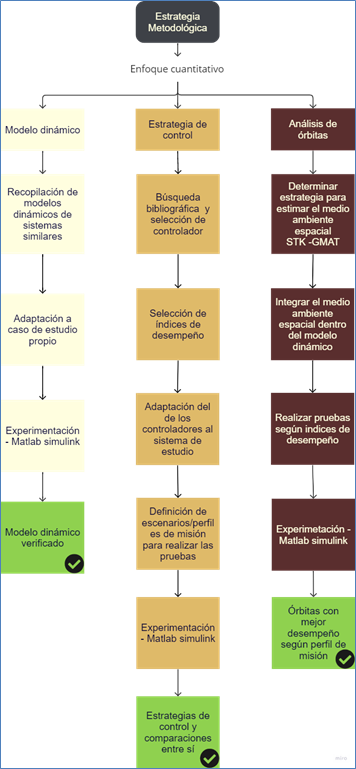
\includegraphics[scale=1]{imagenes/metodologia/grafico_metodologia.png}\\
	\end{center}
	\caption{Diagrama estrategia metodológica}
	\label{fig:metodologia}
	\textit{}
\end{figure}

\FloatBarrier

\section{MODELO DINÁMICO}

La de actitud de una nave espacial como un CubeSat puede ser representada por las ecuaciones dinámicas de Newton-Euler, las cuales describen los efectos de los torques externos e internos que modifican la aceleración del satélite. Para llegar a dichas ecuaciones se parte de la dinámica rotacional tal como se describen en \cite{Griffin2004}.

\begin{figure}[!ht]
	\begin{center}
		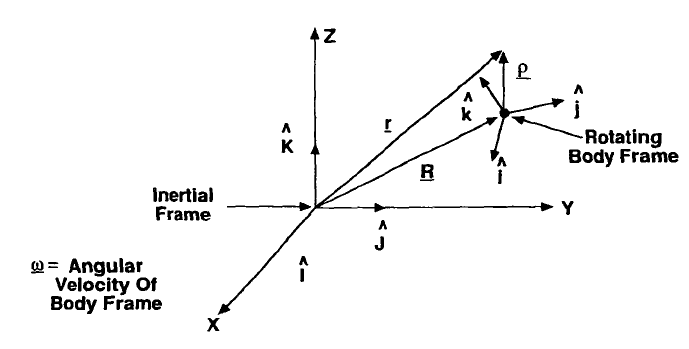
\includegraphics[scale=0.5]{imagenes/modelo_dinamico/ref_system.PNG}\\
	\end{center}
	\caption{Variación en el tiempo de un marco de referencia rotante}
	\label{fig:rot_frame}
	\textit{}
\end{figure}

La Fig.\ref{fig:rot_frame} muestra la geometría esencial del sistema. Se tiene el vector de posición $\rho$ en el marco del cuerpo en rotación, si se desea conocer su variación en el tiempo respecto al marco inercial se tiene:

\begin{equation}\label{eq:variacion_rho}
	\left(\frac{\mathrm{d} \rho}{\mathrm{d} t}\right)_i=\left(\frac{\mathrm{d} \rho}{\mathrm{d} t}\right)_b+\omega \times \boldsymbol{\rho}
\end{equation}

Donde $\omega$ es la velocidad angular en el marco del cuerpo. Por otro lado, se requieren determinar el vector posición $\vec{r}$ y sus derivadas $\vec{v}$ y $\vec{a}$. Del sistema vectorial se tiene una relación entre r y p:

\begin{equation}\label{eq:suma_vectores}
	r = R + \rho
\end{equation}

De esta manera, velocidad y la aceleración pueden ser determinadas: 

\begin{gather}
		\boldsymbol{v}=\left(\frac{\mathrm{d} \boldsymbol{r}}{\mathrm{d} t}\right)_i=\frac{\mathrm{d} \boldsymbol{R}}{\mathrm{d} t}+\left(\frac{\mathrm{d} \boldsymbol{\rho}}{\mathrm{d} t}\right)_b+\omega \times \boldsymbol{\rho}\label{eq:velocidad}\\[10pt]			
		\boldsymbol{a}=\left(\frac{\mathrm{d}^2 \boldsymbol{r}}{\mathrm{d} t^2}\right)_i=\frac{\mathrm{d}^2 \boldsymbol{R}}{\mathrm{d} t^2}+\left(\frac{\mathrm{d}^2 \boldsymbol{\rho}}{\mathrm{d} t^2}\right)_b+2 \omega \times\left(\frac{\mathrm{d} \boldsymbol{\rho}}{\mathrm{d} t}\right)_b+\frac{\mathrm{d} \omega}{\mathrm{d} t} \times \boldsymbol{\rho}+\omega \times(\omega \times \boldsymbol{\rho})\label{eq:aceleracion}				
\end{gather}

En la dinámica rotacional, dos cantidades fundamentales de interés son el momento de inercia y el momento angular. El momento angular de una colección de puntos de masa es el momento de su momento lineal alrededor de un origen definido. A partir de Fig.\ref{fig:rot_frame}, el momento angular de la masa mi alrededor del origen en el sistema de inercial es:

\begin{equation}
	H_{t}=\sum r_i \times m_i v_i\\
\end{equation}

Si aplicamos las eq.(\ref{eq:velocidad}) y eq.(\ref{eq:aceleracion}) con $V =\frac{\mathrm{d} {R}}{\mathrm{d} t}$ y si suponemos que 1) el origen del marco de rotación se encuentra en el centro de masa del cuerpo ($\sum m_i\rho_i =0$), y 2) los vectores de posición $\rho_i$ están fijos en el marco del cuerpo, es decir, tenemos un cuerpo rígido $\frac{\mathrm{d} {\rho}}{\mathrm{d} t} =0$ . Se obtiene el momento angular total así:

\begin{equation}\label{eq:H_total}
H_{t}=\left(\sum m_i\right)R\times V +\sum m_i \rho_i\times\frac{\mathrm{d} {\rho_i}}{\mathrm{d} t} = H_{orb} + H_b \\
\end{equation}

El primer término de la derecha es el momento angular del cuerpo rígido debido a su velocidad traslacional V en el marco de inercia. El segundo término es el momento angular del cuerpo debido a su velocidad de rotación alrededor de su propio centro de masa. La eq. (\ref{eq:H_total}) provee un importante resultado ya que indica que, en un cuerpo rígido, es posible escoger un marco de coordenadas que desacopla el momento angular del cuerpo y del momento angular orbital.
Por tal motivo, el análisis se centrará únicamente en el segundo término, donde la eq.(\ref{eq:variacion_rho}) se simplificaría de la siguiente manera: 

\begin{equation}\label{eq:variacion_rho_simplificada}
	\frac{\mathrm{d} \rho_j}{\mathrm{d} t}=\omega\times\rho_i
\end{equation}

De esta manera, a partir de la eq.(\ref{eq:H_total}) tenemos que el momento angular en el marco del cuerpo es:

\begin{equation}\label{eq:H_total_simplificada}
	H=\sum m_i\rho_i\times\frac{\mathrm{d} {\rho_i}}{\mathrm{d} t} =
	 \sum m_i\rho_i \times(\omega \times \rho_i) = I\omega \\
\end{equation}
Donde $I$ es una matriz real y simétrica, llamada matriz de inercia, con componentes: 
 
 $$
 \begin{aligned}
 	& I_{11}=\sum m_i\left(\rho_{i 2}^2+\rho_{i 3}^2\right) \\
 	& I_{22}=\sum m_i\left(\rho_{i 1}^2+\rho_{i 3}^2\right) \\
 	& I_{33}=\sum m_i\left(\rho_{i 1}^2+\rho_{i 2}^2\right) \\
 	& I_{12}=I_{21}=-\sum m_1 \rho_{i 1} \rho_{i 2} \\
 	& I_{13}=I_{31}=-\sum m_i \rho_{i 1} \rho_{i 3} \\
 	& I_{23}=I_{32}=-\sum m_i \rho_{i 2} \rho_{i 3}
 \end{aligned}
 $$
 
 La eq.(\ref{eq:H_total_simplificada}) nos indica que el momento angular total depende de la matriz de inercia del cubesat y del vector de velocidades angulares. Sin embargo, es necesario introducir el efecto de las ruedas de reacción, las cuales también disponen de un momento angular $h_w$. Por lo tanto, se tiene a partir de la eq.(\ref{eq:H_total_simplificada}) que: 
 
 \begin{equation}\label{eq:H_total_RW}
 	H = I\omega_b + h_w
 \end{equation}
 
 Por otro lado, el efecto de los torques externos se incluye al considerar una fuerza $F_i$ aplicada en una posición $\rho_i$ en las coordenadas del marco del cuerpo. Esta fuerza tiene un efecto dado por: 
  
 \begin{equation}
 	T_i=\rho_i \times F_i  
 \end{equation}
 
 
En este sentido, el torque neto de fuerzas externas es:

\begin{equation}
	T=\sum \rho_i \times F_i=\sum \rho_i \times m_i \frac{\mathrm{d}^2 r_i}{\mathrm{~d} t^2} 	
\end{equation}
 
 
 Al expandir la expresión para la aceleración tal como se hizo en la eq.(\ref{eq:aceleracion}), se tiene que :
 
 \begin{equation}
 	T= \frac{\mathrm{d} H}{\mathrm{d} t} = \left(\frac{\mathrm{d} H}{\mathrm{d} t}\right)_{body} + \omega \times H 	
 \end{equation}
 
 O visto de otra manera, asumiendo un marco fijo del cuerpo con ejes principales, se puede expresar el cambio del momento angular como el efecto de los torques y el producto cruz entre la velocidad angular y el momento angular total del sistema.
 
  \begin{equation}\label{eq:H_dot_1}
 	 \left(\frac{\mathrm{d} H}{\mathrm{d} t}\right)_{body} = T-\omega \times \left(I\omega + h_w\right) 	
 \end{equation}
 
 Análogamente, se puede obtener otra expresión para el cambio de momento angular al derivar la eq.(\ref{eq:H_total_RW}) respecto al tiempo :
 
 \begin{equation}\label{eq:H_dot_2}
 	\dot{H_b} = \left(\frac{\mathrm{d} H}{\mathrm{d} t}\right)_{body} = 
 	I\frac{\mathrm{d} \omega_b}{\mathrm{d} t} + \dot{h_w}  	
 \end{equation}
 
Tomando el principio del intercambio de momentos, se tiene que el momento angular producido por las ruedas de reacción se aplica al satélite con signo opuesto. Entonces si definimos $T_c$ como el par de control:

\begin{equation}
	\dot{h_w} = -T_c  	
\end{equation}

Al igualar las ecuaciones (\ref{eq:H_dot_1}) y (\ref{eq:H_dot_2}) se obtiene una expresión para las aceleraciones angulares, conocida como ecuación dinámica de Newton-Euler, la cual consolida el modelo dinámico del CubeSat:


\begin{equation}\label{eq:modelo_dinamico}
	\frac{d \omega_b}{d t}=I^{-1}\left[-\omega_b \times\left(I \omega_b+h_w\right)+T+T_C\right]	
\end{equation}

donde:
$$
\mathbf{I}=\left[\begin{array}{ccc}
	I_{x x} & I_{x y} & I_{x z} \\
	I_{y x} & I_{y y} & I_{y z} \\
	I_{z x} & I_{z y} & I_{z z}
\end{array}\right]:\text { Matriz de inercia del CubeSat }
$$
$\mathbf{\omega_b}=\left[\begin{array}{l}\omega_x \\ \omega_y \\ \omega_z\end{array}\right]:$ Vector de velocidad angular del satélite en el marco del cuerpo.\\

$\mathbf{h_w}=\left[\begin{array}{l}h_x \\ h_y \\ h_z\end{array}\right]:$ Vector de momento de angular de las RW. 

Realizando las respectivas multiplaciones matriciales, se tienen las ecuaciones en cada eje:

\begin{gather}	
	\dot{\omega}_x=\left[T_x+T_{C x}+\omega_y \omega_z\left[I_{y y}-I_{z z}\right]-h_z \omega_y+h_y \omega_z\right] / I_{x x}\label{eq:modelo_dinamico_x}\\
	\dot{\omega}_y=\left[T_y+T_{C y}+\omega_x \omega_z\left[I_{z z}-I_{x x}\right]-h_x \omega_z+h_z \omega_x\right] / I_{y y}\label{eq:modelo_dinamico_y}\\
	\dot{\omega}_z=\left[T_z+T_{C z}+\omega_x \omega_y\left[I_{x x}-I_{y y}\right]-h_y \omega_x+h_x \omega_y\right] / I_{z z}
\end{gather}




Finalmente, usando las componentes del vector de velocidades angulares es posible determinar la actitud del CubeSat. La interpretación de los ángulos de Euler es más intuitiva, pero para evitar que surjan singularidades, los cuaterniones
resultan mas convenientes para los cálculos de simulación \cite{Steyn2011}. La ecuación diferencial cinemática de los cuaterniones está descrita en la eq.(\ref{eq:quaterniones}): 

\begin{equation}\label{eq:quaterniones}
	\dot{\mathbf{q}}=\frac{1}{2} \Omega \mathbf{q} \\
\end{equation}

Donde
 
\begin{center}
 	$\Omega$ = $\left[\begin{array}{cccc}
 		0 & w_z & -w_y & w_x \\
 		-w_z & 0 & w_x & w_y \\
 		w_y & -w_x & 0 & w_z \\
 		-w_x & -w_y & -w_z & 0
 	\end{array}\right]$ 
 	
\end{center}
\hspace{\parindent} y
\begin{center}
	$
	\mathbf{q}=\left[\begin{array}{llll}
		q_1 & q_2 & q_3 & q_4
	\end{array}\right]^T
	$
\end{center}


%% Fuerzas externas

%Aerodinámica
% Magnetorques


\newpage
%--------------------------
\section{RESULTADOS}

En los resultados se comunican los hallazgos y descubrimientos del estudio. Se incluyen tablas, figuras, diagramas y demás material demostrativo.




 Al narrar descriptivamente una figura, tabla, etc., en un párrafo, puedes insertar una referencia cruzada, es decir, un hipervínculo al elemento mencionado dentro o fuera de paréntesis, ejemplos: estos resultados se muestran en la \textbf{Tabla \ref{table:prob_milenio}}.  Igualmente, los datos son validados con otros instrumentos \textbf{(Tabla \ref{table:num_mersenne}, Tabla \ref{table:medalla_fields})}. Lineamientos que se establecen en la nueva versión de las Normas APA séptima edición \textbf{(Fig. \ref{figportada_apa})}. La producción intelectual institucional se publica en el Repositorio \textbf{(Fig. \ref{fig:escudo_udea})}. Si la figura es de tu completa autoría, \textbf{NO} es necesario colocar la leyenda “Elaboración propia” \textbf{(Fig. \ref{fig:hiperbolica})}.

\begin{figure}[!ht]
    \begin{center}
    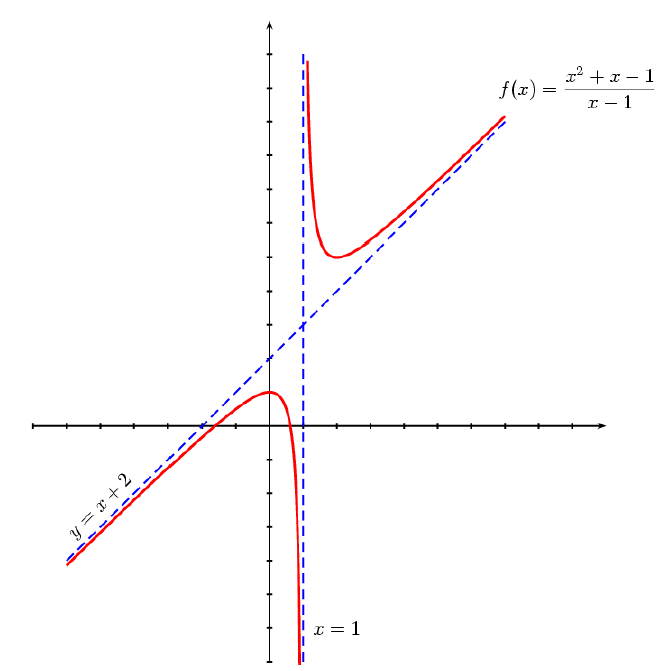
\includegraphics[scale=0.5]{imagenes/grafica.png}\\
    \end{center}
    \caption{Función hiperbólica}
    \label{fig:hiperbolica}
    \textit{}
\end{figure}

\begin{table}%[!ht]
\caption{\MakeUppercase{Problemas del milenio: la resolucion de uno de estos problemas se premian con un monto de us\$ 1 millon}}
\begin{center}
\begin{tabular}{  l c }
    \hline
    1 & El problema de $P$ frente a $NP$  \\ \hline
    2 &  La conjetura de Hodge \\ \hline
    3 &  La conjetura de Poincaré \\ \hline
    4 &  La hipótesis de Riemann \\ \hline
    5 &  Yang-Mills y el salto de masa ("mass gap")\\ \hline
    6 &  Las ecuaciones de Navier-Stokes\\ \hline
    7 &  Conjetura de Birch y Swinnerton-Dyer\\
        \hline
\end{tabular}
\end{center}
\label{table:prob_milenio}
\end{table}

%\clearpage

\begin{table}%[!ht]
\caption{\MakeUppercase{Medalla Fields: matemáticos galardonados con este premio desde 2010; la medalla Fields se comenzó a entregar desde 1936}}
\begin{center}
\begin{tabular}{cp{4cm}p{2.5cm}p{6cm}}
    \hline
    año & Ganador(es) & pais & universidad/instituto\\
    \hline 
        2010 & Elon Lindenstrauss & Israel & Universidad Hebrea de Jerusalén\\
         & Ngo Bao Chau ,  & Vietnam y Francia &Paris-Sud 11 University y Institute for Advanced Study \\
         & Stanislav Smirnov  & Rusia & Universidad de Ginebra\\
         & Cédric Villani & Francia & Institut Henri Poincaré\\
         \hline
         2014 & Artur Ávila  & Francia &Instituto Nacional de Matemática Pura y Aplicada \\
         & Manjul Bhargava  &  Canadá y Estados Unidos &Universidad de Princeton \\
         & Martin Hairer & Austria & Imperial College London\\
         & Maryam Mirzajani & Irán &Universidad Stanford \\
         \hline\\
         2018	 & Caucher Birkar & Irán y Reino Unido & Universidad de Cambridge \\
         & Alessio Figalli & Italia & Escuela Politécnica Federal de Zúrich \\
         & Peter Scholze & Alemania & Universidad de Bonn\\
         & Akshay Venkatesh  & Australia & Universidad Stanford\\
        \hline
\end{tabular}
\end{center}
\label{table:medalla_fields}
\end{table}

\clearpage

\begin{table}%[!ht]
\caption{\MakeUppercase{Algunos números primos de Mersenne}}
\begin{center}
\begin{tabular}{ c|c}
    \hline
    Exponente $n$ & Primo de Mersenne \\ \hline
    2 &  $2^{2}-1=3 $ \\ \hline
    3 &  $2^{3}-1=7 $ \\ \hline
    5 &  $2^{5}-1=31 $ \\ \hline
    7 &  $2^{7}-1=127 $ \\ \hline
    13 &  $2^{13}-1=8191 $ \\ \hline
    17 &  $2^{17}-1=131071 $ \\
        \hline
\end{tabular}
\end{center}
\label{table:num_mersenne}
\end{table}


\begin{figure}[!ht]
    \begin{center}
    
\includegraphics[scale=0.5]{imagenes/ieee_logo.jpg}\\
    \end{center}
    \caption{Imagen corporativa Institute of Electrical and Electronics Engineers (IEEE)}
    \label{figportada_apa}
    \footnotesize{Nota. Fuente \url{https://www.ieee.org/} Esta entidad edita y normaliza la presentación de documentos científicos en el área de ingenierías.} %\citep{lib:apa}.
\end{figure}

\clearpage

\begin{figure}[!ht]
    \begin{center}
    
\includegraphics{imagenes/escudo_udea_solo.png}\\
    \end{center}
    \caption{Logo Universidad de Antioquia}
    \label{fig:escudo_udea}
    \footnotesize{Nota. Fuente \url{http:/www.udea.edu.co}}
\end{figure}

\clearpage

%--------------------------
\section{DISCUSIÓN}

La discusión es la interpretación crítica y el análisis de los resultados, que surgen de las preguntas de investigación.


\newpage
%--------------------------
\section{CONCLUSIONES}

Son las interpretaciones finales que recopilan los datos de la investigación, describe lo que se obtuvo, qué se logró y cuáles son los resultados. Guardan relación directa con lo que se mencionó en el planteamiento del problema. Pueden confirmar las hipótesis. 


\newpage
%--------------------------
\section{RECOMENDACIONES}

Las recomendaciones son las futuras y posibles líneas de investigación que llevarán a resolver problemas relacionados con la presente investigación.


